\documentclass[11pt,a4paper]{article}
\usepackage[margin=2.5cm]{geometry}
\usepackage{fontspec}
\usepackage{array}
\usepackage{booktabs}
\usepackage{tabularx}
\usepackage{multirow,graphicx}
\usepackage{parskip}
\usepackage[table]{xcolor}
\definecolor{lightgrey}{gray}{0.9}

% Set main font to Sorts Mill Goudy
\setmainfont{Sorts Mill Goudy}

% Define column types
\newcolumntype{T}{>{\raggedright\arraybackslash}p{3cm}}
\newcolumntype{S}{>{\raggedright\arraybackslash}X}

\begin{document}

\begin{center}
    {\LARGE Issues in Phonological Typology @ UiT} \\
    {\large \textcolor{red}{Draft programme — 22 October 2025}}
\end{center}

\textsc{Location.} Fakultet for Humaniora, Samfunnsvitenskap og Lærerutdanning, room E0103 (talks) and the mezzanine between B and D wing (posters). 

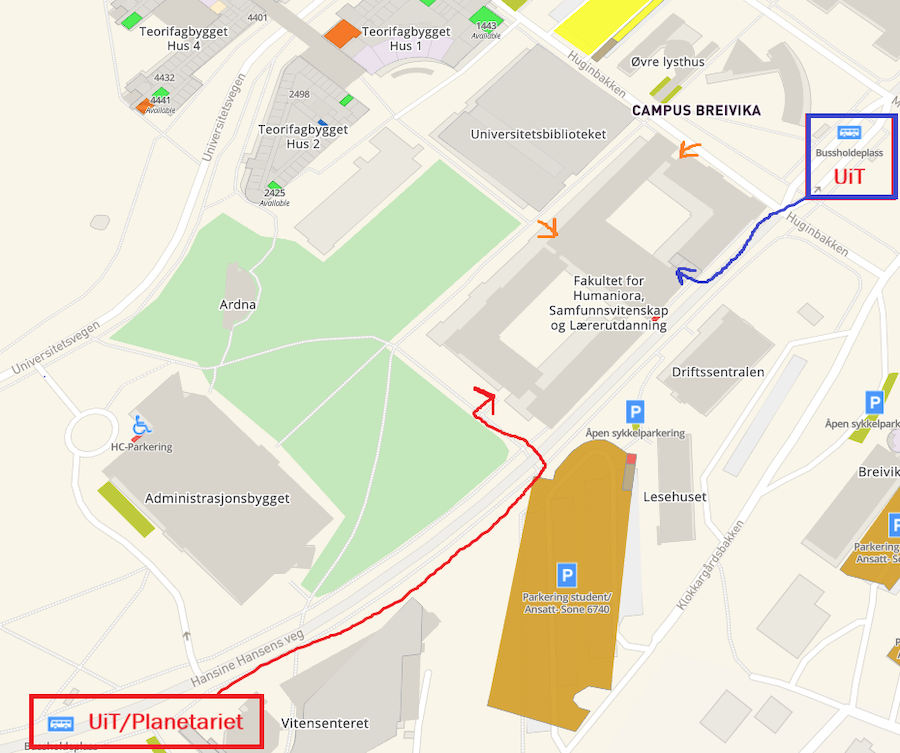
\includegraphics[width=0.5\textwidth]{map.png}
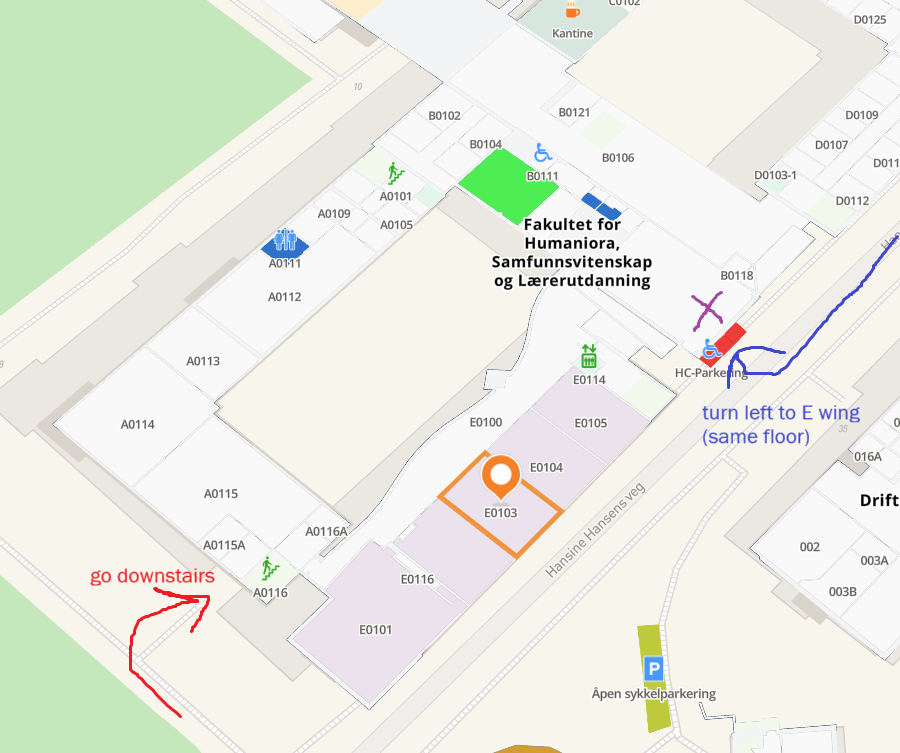
\includegraphics[width=0.5\textwidth]{map2.png}

\vspace{1cm}

\begin{center}
    {\Large Schedule}
\end{center}

{\large Thursday 27 November}

\noindent
\begin{tabularx}{\textwidth}{T S}
\toprule
\textbf{Time} & \textbf{Session} \\
\midrule
09:00--09:15 & \textbf{Welcome} \\
\midrule
09:15--10:00 & Birgit Alber \& Nick Kalivoda \\
& \textit{An exploration of grammatical adjacency} \\
\midrule
10:00--10:45 & Eirini Apostolopoulou \\
& \textit{Coda inventories and typological variation in Italiot Greek} \\
\midrule
\rowcolor{lightgrey}
10:45--11:15 & \textbf{Coffee Break} \\
\midrule
11:15--12:00 & Jahnavi Narkar \\
& \textit{A probabilistic model of stop inventory typology}  \\
\midrule
12:00--12:45 & Michael Dow \\
& \textit{A clustering analysis of nasal vs. oral vowel inventories}  \\
\midrule
\rowcolor{lightgrey}
12:45--14:00 & \textbf{Lunch} \\
\midrule
14:00--14:45 & Roland Noske \\
& \textit{Typological evolutionary paths}  \\
\midrule
14:45--15:30 & Alan Avdagic \& Håvard Weiberg Johansen \\
& \textit{The evolution of vertical vowel systems}  \\
\midrule
\rowcolor{lightgrey}
15:30--16:00 & \textbf{Coffee Break} \\
\midrule
\rowcolor{cyan!10}
16:00--17:00 & \textbf{Invited Talk:} Joachim Kokkelmans \\
\rowcolor{cyan!10}
& \textit{Obstruent inventories: gaps, universals and simulations}  \\
\bottomrule
\end{tabularx}

\vspace{1.5cm}

{\large Friday 28 November}

\noindent
\begin{tabularx}{\textwidth}{T S}
\toprule
\textbf{Time} & \textbf{Session} \\
\midrule
09:15--10:00 & Martin Krämer \& Draga Žec \\
& \textit{A typology of syllabic consonants: how variable is their vocalic nature?}  \\
\midrule
10:00--10:45 & Ryan Chon \\
& \textit{Invoking typology to account for phonological asymmetries in Yuhup and Hup} \\
\midrule
\rowcolor{lightgrey}
10:45--11:15 & \textbf{Coffee Break} \\
\midrule
11:15--12:00 & Péter Őri \\
& \textit{Phonological vs. phonetic typologies of laryngeal systems}  \\
\midrule
12:00--12:45 & Ruben Roberto Peralta Rivera \\
& \textit{Gradient Integration of Anglicisms in Bilingual Speech: A Phonetic-Typological Approach}  \\
\midrule
\rowcolor{lightgrey}
12:45--14:00 & \textbf{Lunch} \\
\midrule
14:00--14:45 & Jenna Conklin \& Martin Krämer \\
& \textit{Challenges and Advantages in Using Artificial Grammar Learning to Expand Natural Typologies}  \\
\midrule
\rowcolor{yellow!20}
14:45--16:00 & \textbf{Poster Session \& Coffee} \\
& Letizia Cerqueglini \\
& \textit{Exploring the Prosody-Morphology Interface: A Typological Assessment of Mutallat Arabic Pausal Forms}  \\ \\
& Pratikshya Guru \\
& \textit{Experimental Method in understanding Empty Nuclei and Rhymal Coda}  \\ \\
& Alireza Jaferian \\
& \textit{A typological tool for marginal consonant clusters}  \\ \\
& Giorgos Markopoulos \& Anthi Revithiadou \\
& \textit{Lexical stress with gradient Theme prominence: A typological perspective}  \\ \\
& Elena Perekhvalskaya \& Valentin Vydrin \\
& \textit{Tonal density index as a yardstick to the functional load of tone}  \\ \\
& Valentin Vydrin \& Kirill Maslinsky \\
& \textit{Towards a typology of tone}  \\ \\
& Andrew Wedel \\
& \textit{Chain Shifts and Transphonologizations are Driven by Homophony Avoidance} \\
\midrule
\rowcolor{cyan!10}
16:00--17:00 & \textbf{Invited Talk:} Sara Finley \\
\rowcolor{cyan!10}
& \textit{Teasing apart learning and processing biases in phonological typology}  \\
\midrule
17:00--17:30 & \textbf{Wrap-up} \\
\midrule
\textcolor{red}{17:30--} & \textcolor{red}{\textbf{Workshop Dinner}, exact time and place to be announced.}\\
\bottomrule
\end{tabularx}

\end{document}